\begin{refsection}
\chapter{How Can Multigrid Fail?}

If the coarse space cannot capture modes not handled by the smoother, then those error components will not be reduced and the convergence will stall. Thus, we would like to have a way to monitor the quality of the coarse space. To do this, we run the process in reverse. Suppose that I had the exact solution in the coarse space. I would prolong this into the original fine space and then run the smoother. If the error is reduced quickly, without disturbing the coarse solution, then the smoother is working well. In short, if we smooth in the complement of the coarse space, we should see good convergence. This kind of smoothing is called \defineTerm{compatible relaxation}~\parencite{Brandt2000,BrannickFalgout2007}, and one cycle can be written
\begin{align}
  \vb{v}_{k+1} = \left( I - S (S^T M S)^{-1} S^T A \right) \vb{v}_k.
\end{align}
Since $R S = 0$, we can write the whole thing as
\begin{align}
  \vb{v}_{k+1} = \left( I - M_S^{-1} A_S \right) \vb{v}_k.
\end{align}
where $A_S = S^T A S$ and likewise for $M$, as shown in~\parencite{BrannickEtAl2018}.

\section{Anisotropic Coefficient}

We will start solving this problem with our standard GMG solver,
\begin{bash}
./poisson -coeff_type anisotropic -k -1
  -potential_petscspace_degree 1 -dm_plex_box_faces 16,16 -dm_refine_hierarchy 6
  -ksp_type cg -ksp_rtol 1e-10
  -pc_type mg -mg_levels_ksp_max_it 2 -mg_levels_pc_type jacobi
    -mg_levels_esteig_ksp_type cg -mg_levels_esteig_ksp_max_it 10 -mg_levels_ksp_chebyshev_esteig 0,0.05,0,1.05
  -ksp_monitor_error draw::draw_lg -ksp_monitor_pause_final
\end{bash}
If the difference in the values for $x$ and $y$ is only one order of magnitude, then our convergence is basically unchanged
\begin{bash}
0 SNES Function norm 3.215985340573e+02   Rate
  0 KSP Residual norm 9.862882847633e+02
  1 KSP Residual norm 1.067418792425e+02  0.11
  2 KSP Residual norm 1.170787252211e+01  0.11
  3 KSP Residual norm 3.220190329561e+00  0.28
  4 KSP Residual norm 3.697605469473e-01  0.11
  5 KSP Residual norm 9.800443978108e-02  0.26
  6 KSP Residual norm 2.048479959211e-02  0.21
  7 KSP Residual norm 3.552256547716e-03  0.17
  8 KSP Residual norm 7.635109560268e-04  0.21
  9 KSP Residual norm 1.621948714165e-04  0.21
 10 KSP Residual norm 2.320226509599e-05  0.14
 11 KSP Residual norm 4.346694615058e-06  0.19
 12 KSP Residual norm 9.341461114587e-07  0.10
 13 KSP Residual norm 1.230311675666e-07  0.13
 14 KSP Residual norm 2.252822538750e-08  0.18
1 SNES Function norm 2.072530386954e-08
\end{bash}
However, if we increase $k$, the number of iterations increases drastically until we hit $k = 4$, after which it stays roughly constant, as can bee seen in Fig.~\ref{fig:errorAnisoK}. We can also see that multigrid is losing its scalability, in that as I increase the mesh size the contraction rate is falling
\begin{bash}
  ./poisson -dm_refine_hierarchy 2 -k -4 -coeff_type anisotropic ...
    -ksp_converged_rate -ksp_converged_rate_type residual
  Linear solve converged due to CONVERGED_RTOL iterations 72 res rate 0.767723 R^2 0.976486
  ./poisson -dm_refine_hierarchy 4 -k -4 -coeff_type anisotropic ...
    -ksp_converged_rate -ksp_converged_rate_type residual
  Linear solve converged due to CONVERGED_RTOL iterations 203 res rate 0.914207 R^2 0.973331
  ./poisson -dm_refine_hierarchy 6 -k -4 -coeff_type anisotropic ...
    -ksp_converged_rate -ksp_converged_rate_type residual
  Linear solve converged due to CONVERGED_RTOL iterations 298 res rate 0.940867 R^2 0.993658
\end{bash}
and the number of iterates to hit discretization error increases, as shown in Fig.~\ref{fig:errorAnisoN}. So what is going wrong?

\begin{figure}
\centering
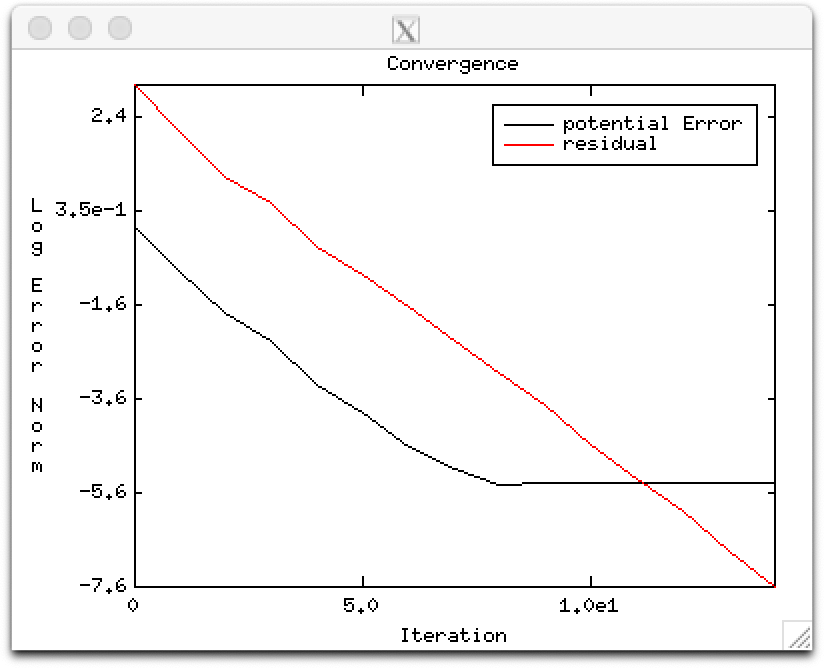
\includegraphics[width=2in]{figures/errorAnisoK1_r6.png}\hfil
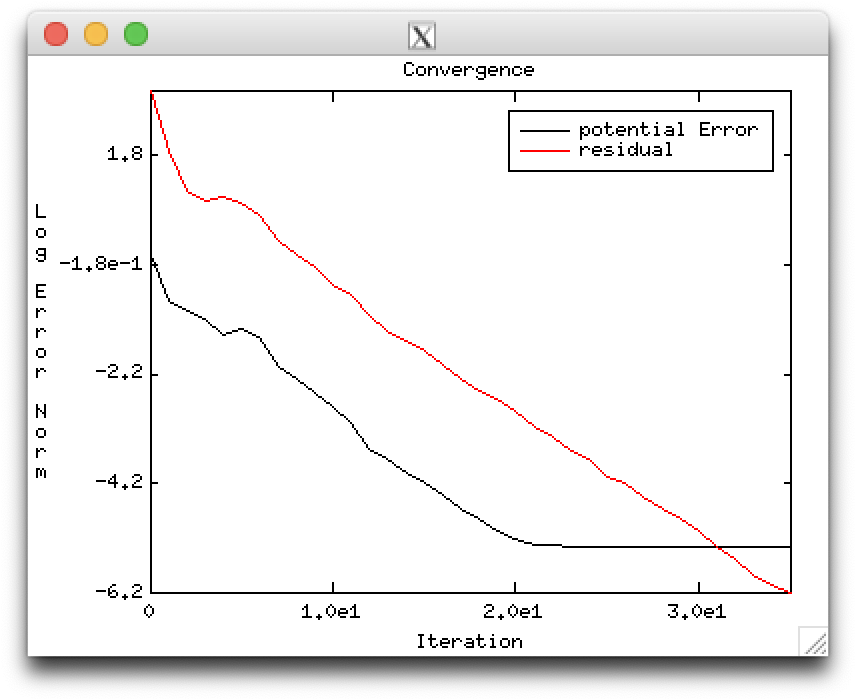
\includegraphics[width=2in]{figures/errorAnisoK2_r6.png}\\
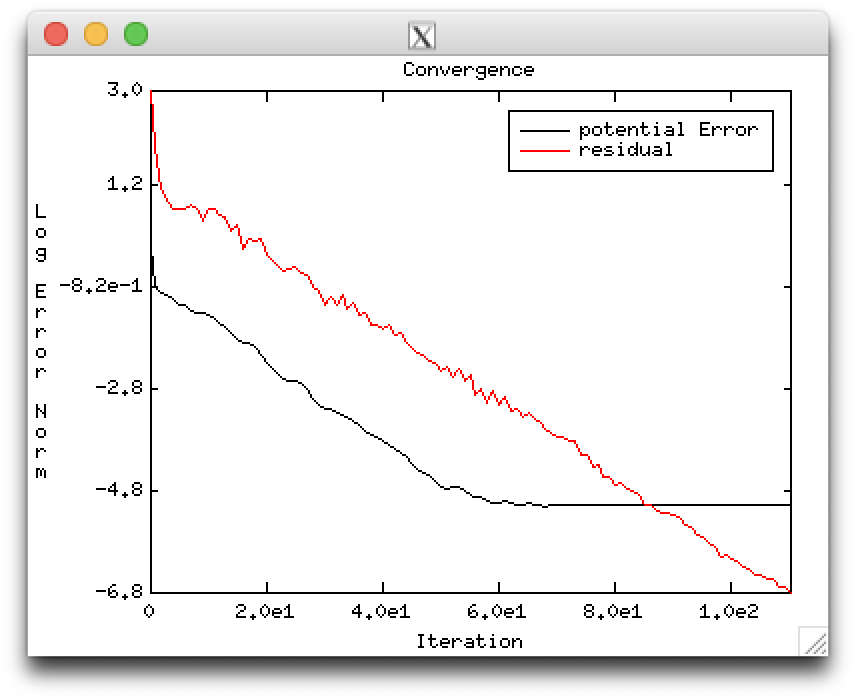
\includegraphics[width=2in]{figures/errorAnisoK3_r6.png}\hfil
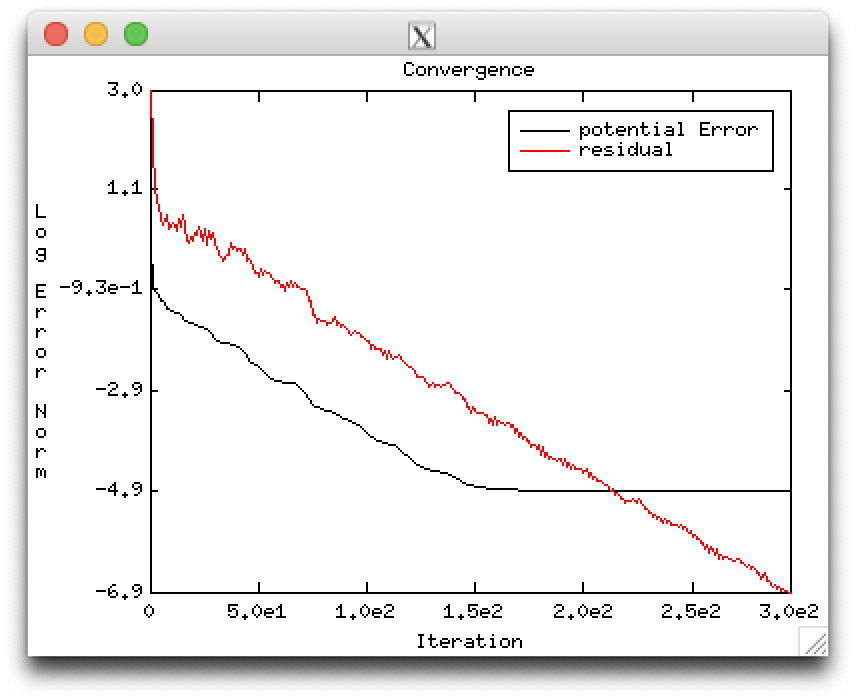
\includegraphics[width=2in]{figures/errorAnisoK4_r6.png}
\caption{Plot of error and residual norms for each iterate of our multigrid solve for $k$ = -1, -2, -3, and -4.\label{fig:errorAnisoK}}
\end{figure}

\begin{figure}
\centering
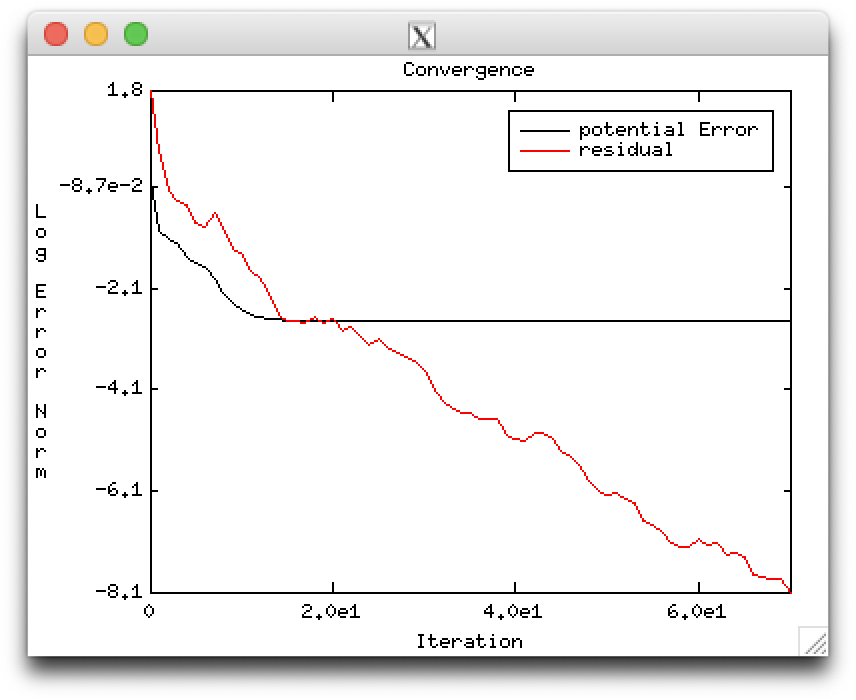
\includegraphics[width=1.5in]{figures/errorAnisoK4_r2.png}\hfil
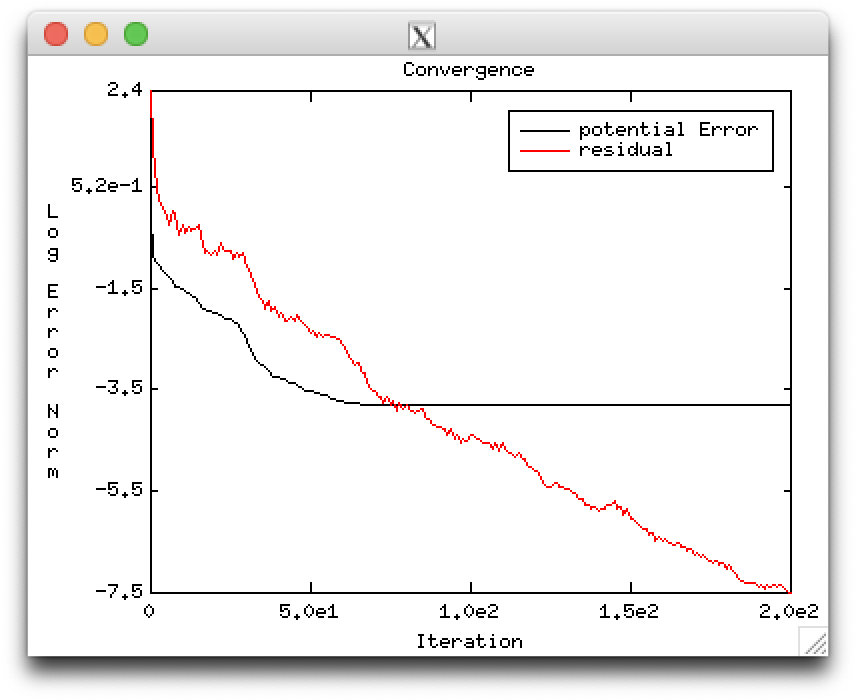
\includegraphics[width=1.5in]{figures/errorAnisoK4_r4.png}\hfil
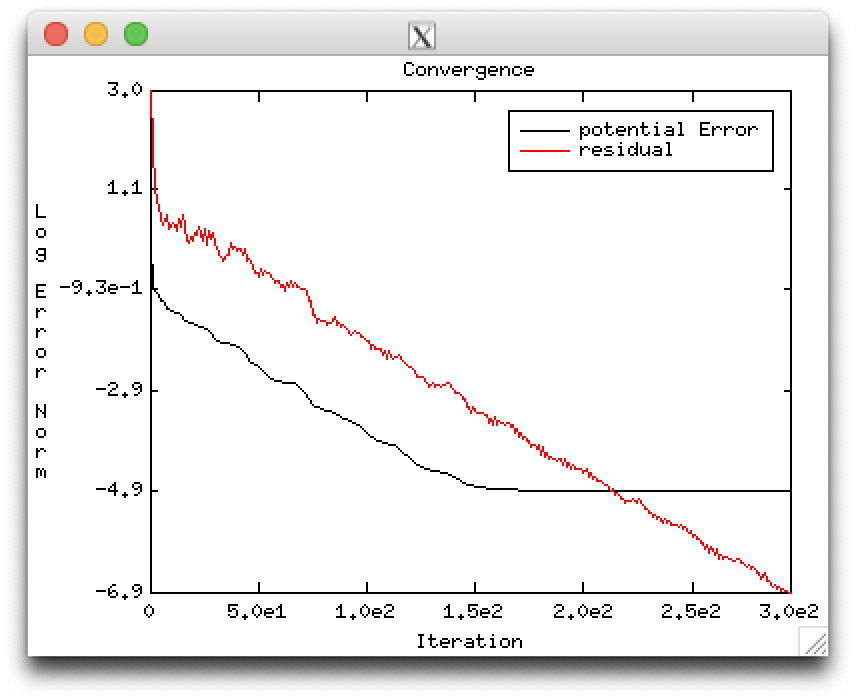
\includegraphics[width=1.5in]{figures/errorAnisoK4_r6.png}
\caption{Plot of error and residual norms for each iterate of our multigrid solve with $k$ = -4 for 2, 4, and 6 refinements of the initial mesh.\label{fig:errorAnisoN}}
\end{figure}

We can first try to see if our smoother has become less effective using the rate monitor on our first level.
\begin{bash}
  ./poisson -dm_refine_hierarchy 2 -k -4 -coeff_type anisotropic ...
    -mg_levels_1_ksp_converged_rate -mg_levels_1_ksp_converged_rate_type residual
    -mg_levels_1_ksp_norm_type preconditioned
      Linear mg_levels_1_ solve converged due to CONVERGED_ITS iterations 2 res rate 0.721296 R^2 0.992187
      Linear mg_levels_1_ solve converged due to CONVERGED_ITS iterations 2 res rate 0.680885 R^2 0.98317
      Linear mg_levels_1_ solve converged due to CONVERGED_ITS iterations 2 res rate 0.616259 R^2 0.974962
      Linear mg_levels_1_ solve converged due to CONVERGED_ITS iterations 2 res rate 0.732815 R^2 0.992424
      Linear mg_levels_1_ solve converged due to CONVERGED_ITS iterations 2 res rate 0.764227 R^2 0.996241
      ...
      Linear mg_levels_1_ solve converged due to CONVERGED_ITS iterations 2 res rate 0.870409 R^2 0.979988
      Linear mg_levels_1_ solve converged due to CONVERGED_ITS iterations 2 res rate 0.812481 R^2 0.999999
      Linear mg_levels_1_ solve converged due to CONVERGED_ITS iterations 2 res rate 0.816343 R^2 0.993959
      Linear mg_levels_1_ solve converged due to CONVERGED_ITS iterations 2 res rate 0.807783 R^2 0.999019
      Linear mg_levels_1_ solve converged due to CONVERGED_ITS iterations 2 res rate 0.834384 R^2 0.998993
\end{bash}
It starts out fine, and gets slightly worse, so we might suspect that it is not the smoother itself which is to blame, but rather the combination of the smoother and coarse space. We can test this using our CR monitor.
\begin{bash}
  ./poisson -dm_refine_hierarchy 2 -k -4 -coeff_type anisotropic ...
    -pc_mg_adapt_cr -mg_levels_cr_ksp_max_it 5 -mg_levels_cr_ksp_converged_rate
    -mg_levels_cr_ksp_converged_rate_type error
      Linear mg_levels_1_cr_ solve converged due to CONVERGED_ITS iterations 5 error rate 0.753441 R^2 0.950102
    Linear mg_levels_2_cr_ solve converged due to CONVERGED_ITS iterations 5 error rate 0.762209 R^2 0.925055
    ...
  ./poisson -dm_refine_hierarchy 4 -k -4 -coeff_type anisotropic ...
    -pc_mg_adapt_cr -mg_levels_cr_ksp_max_it 5 -mg_levels_cr_ksp_converged_rate
    -mg_levels_cr_ksp_converged_rate_type error
          Linear mg_levels_1_cr_ solve converged due to CONVERGED_ITS iterations 5 error rate 0.753441 R^2 0.950102
        Linear mg_levels_2_cr_ solve converged due to CONVERGED_ITS iterations 5 error rate 0.762209 R^2 0.925055
      Linear mg_levels_3_cr_ solve converged due to CONVERGED_ITS iterations 5 error rate 0.762132 R^2 0.914645
    Linear mg_levels_4_cr_ solve converged due to CONVERGED_ITS iterations 5 error rate 0.766149 R^2 0.916249
  ./poisson -dm_refine_hierarchy 6 -k -4 -coeff_type anisotropic ...
    -pc_mg_adapt_cr -mg_levels_cr_ksp_max_it 5 -mg_levels_cr_ksp_converged_rate
    -mg_levels_cr_ksp_converged_rate_type error
              Linear mg_levels_1_cr_ solve converged due to CONVERGED_ITS iterations 5 error rate 0.753441 R^2 0.950102
            Linear mg_levels_2_cr_ solve converged due to CONVERGED_ITS iterations 5 error rate 0.762209 R^2 0.925055
          Linear mg_levels_3_cr_ solve converged due to CONVERGED_ITS iterations 5 error rate 0.762132 R^2 0.914645
        Linear mg_levels_4_cr_ solve converged due to CONVERGED_ITS iterations 5 error rate 0.766149 R^2 0.916249
      Linear mg_levels_5_cr_ solve converged due to CONVERGED_ITS iterations 5 error rate 0.768881 R^2 0.914111
    Linear mg_levels_6_cr_ solve converged due to CONVERGED_ITS iterations 5 error rate 0.767963 R^2 0.913506
\end{bash}
whereas for a fully functioning multigrid we get
\begin{bash}
  ./poisson -dm_refine_hierarchy 2 -k 0 -coeff_type anisotropic ...
    -pc_mg_adapt_cr -mg_levels_cr_ksp_max_it 5 -mg_levels_cr_ksp_converged_rate
    -mg_levels_cr_ksp_converged_rate_type error
      Linear mg_levels_1_cr_ solve converged due to CONVERGED_ITS iterations 5 error rate 0.671787 R^2 0.960782
    Linear mg_levels_2_cr_ solve converged due to CONVERGED_ITS iterations 5 error rate 0.642287 R^2 0.976622
    ...
  ./poisson -dm_refine_hierarchy 4 -k 0 -coeff_type anisotropic ...
    -pc_mg_adapt_cr -mg_levels_cr_ksp_max_it 5 -mg_levels_cr_ksp_converged_rate
    -mg_levels_cr_ksp_converged_rate_type error
          Linear mg_levels_1_cr_ solve converged due to CONVERGED_ITS iterations 5 error rate 0.671787 R^2 0.960782
        Linear mg_levels_2_cr_ solve converged due to CONVERGED_ITS iterations 5 error rate 0.642287 R^2 0.976622
      Linear mg_levels_3_cr_ solve converged due to CONVERGED_ITS iterations 5 error rate 0.642214 R^2 0.973073
    Linear mg_levels_4_cr_ solve converged due to CONVERGED_ITS iterations 5 error rate 0.646824 R^2 0.974903
  ./poisson -dm_refine_hierarchy 6 -k 0 -coeff_type anisotropic ...
    -pc_mg_adapt_cr -mg_levels_cr_ksp_max_it 5 -mg_levels_cr_ksp_converged_rate
    -mg_levels_cr_ksp_converged_rate_type error
              Linear mg_levels_1_cr_ solve converged due to CONVERGED_ITS iterations 5 error rate 0.671787 R^2 0.960782
            Linear mg_levels_2_cr_ solve converged due to CONVERGED_ITS iterations 5 error rate 0.642287 R^2 0.976622
          Linear mg_levels_3_cr_ solve converged due to CONVERGED_ITS iterations 5 error rate 0.642214 R^2 0.973073
        Linear mg_levels_4_cr_ solve converged due to CONVERGED_ITS iterations 5 error rate 0.646824 R^2 0.974903
      Linear mg_levels_5_cr_ solve converged due to CONVERGED_ITS iterations 5 error rate 0.645552 R^2 0.975915
    Linear mg_levels_6_cr_ solve converged due to CONVERGED_ITS iterations 5 error rate 0.645276 R^2 0.976259
\end{bash}
Thus, it looks like the recommendation by Brannick and Falgout to choose 0.7 as the cutoff for acceptable CR convergence is a good one.

\section{MiniProjects}

Create monitor to show CR error

Create monitor to show difference between projected error with and without coarse adaptation

\printbibliography[heading=subbibliography] % print section bibliography
\end{refsection}
